\documentclass[a4paper]{article}
\usepackage{graphicx}
\usepackage{twocolpceurws}
\usepackage{float}
\usepackage{hyperref}

\title{Using Refactoring Techniques to Reduce Duplication in Object-Oriented Programming Languages}

\author{
Simon Baars \\ University of Amsterdam\\
                Puiflijk, Netherlands \\ simon.mailadres@gmail.com
\and
Ana Oprescu \\ University of Amsterdam\\
                Amsterdam, Netherlands \\ A.M.Oprescu@uva.nl
}

\institution{}


\begin{document}
\maketitle

\begin{abstract}
Duplication in source code can have a major negative impact on the maintainability of source code. There are several techniques that can be used in order to merge clones, reduce duplication and potentially also reduce the total volume of a software system. In this study, we look into the opportunities to aid in the process of refactoring these duplication problems for object-oriented programming languages. Measurements that have been conducted so far have indicated that more than half of the duplication in code is related to each other through inheritance, making it easier to refactor these clones in a clean way. More measurements will be conducted to get a detailed overview of in what contexts clones occur, and what this means for the refactoring processes of these clones. As a desired output, we strive to construct a model that automatically applies refactorings for a large part of the detected duplication problems and implement this model for the Java programming language.
\end{abstract}


\section{Introduction}
Refactoring is used to improve quality related attributes of a codebase (maintainability, performance, etc.) without changing the functionality. There are many methods that have been introduced to help with the process of refactoring \cite{fowler2018refactoring, wake2004refactoring}. However, most of these methods still require manual assessment of where and when to apply them. Because of this, refactoring takes up a signification portion of the development process \cite{lientz1978characteristics, mens2004survey}, or does not happen at all \cite{mens2003refactoring}. For a large part, refactoring requires domain knowledge to do it right. However, there are also refactoring opportunities that are rather trivial and repetitive to execute. In this thesis, we take a look at the challenges and opportunities in automatically refactoring duplicated code, also known as ``code clones''. The main goal is to improve maintainability of the refactored code.

Duplication in source code is often seen as one of the most harmful types of technical debt. In Martin Fowler's ``Refactoring'' book \cite{fowler2018refactoring}, he exclaims that \textit{``Number one in the stink parade is duplicated code. If you see the same code structure in more than one place, you can be sure that your program will be better if you find a way to unify them.''}. However, this statement is not accepted by everyone. Several papers argue that not each type of duplication is harmful \cite{kapser2006cloning}.

In this research, we focus on formalizing the refactoring process of dealing with duplication in code. We will measure open source projects from the We will show the improvement of the metrics over various open source and industrial projects. Likewise, we will perform an estimation of the development costs that are saved by using the proposed solution. We will lay the main focus on the Java programming language as refactoring opportunities do feature paradigm and programming language dependent aspects \cite{choi2011extracting}. However, most practises used in this thesis will also be applicable with other object-oriented languages, like C\#.

\section{Clone Detection}
As duplication in source code is a serious problem in many software systems, there are a lot of researches that look into code clones. Many tools have been proposed to detect various types of code clones. Two surveys of modern clone detection tools \cite{sheneamer2016survey, svajlenko2014evaluating} together show an overview of the most-popular clone detection tools up until 2016. To be able to refactor detected clones, it is useful to have the ability to rewrite the AST. We considered a set of clone detection tools for their ability to support the refactoring process automatically. None of the tools we consider seemed completely fit for this purpose, so we decided to implement our own clone detection tool: CloneRefactor\footnote{CloneRefactor (WIP) is available on GitHub: \url{https://github.com/SimonBaars/CloneRefactor}}.

\subsection{CloneRefactor}
A 2016 survey by Gautam \cite{gautam2016various} focuses more on various techniques for clone detection. For our tool we decided to combine AST and Graph based approaches for clone detection, similar to Scorpio (which is a clone detection tool that's part of TinyPDG: a library for building intraprocedural program dependency graphs for Java programs). We decided to base our tool on the JavaParser library \cite{tomassetti2017javaparser}, as it supports rewriting the AST back to Java code. We then collect each statement and declaration (ommitting their child statements and declarations) and compare those to find duplicates. This way we build a graph of each statement/declaration linking to each subsequent statement/declaration (horizontally) and linking to each of it's duplicates (verically). This is displayed in figure \ref{fig:clonerefactor}.

\begin{figure}[H]
  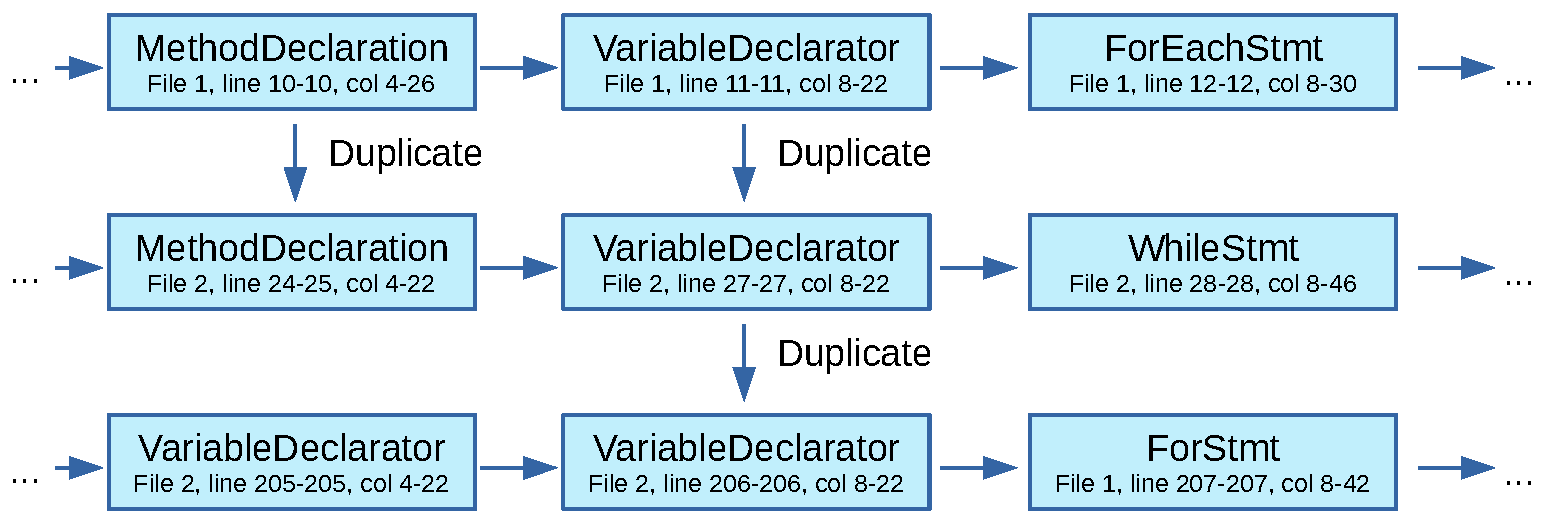
\includegraphics[width=1\columnwidth]{img/CodeGraph}
  \caption{Abstract figure of the graph representation built by CloneRefactor}
  \label{fig:clonerefactor}
\end{figure}

\section{Code Clone Context}
To be able to refactor code clones, it is very important to consider the context of the clone. We define the following aspects of the clone as its context:
\begin{enumerate}
  \item The relation of clone instances among each other (for example: two clone instances in a clone class are part of the same object).
  \item Where a clone instance occurs in the code (for instance: a method-level clone is a clone instance that is (a part of) a single method).
  \item The contents of a clone instance (for instance: the clone instance consists of a one method declaration, a foreach statement and two variable declarations).
\end{enumerate}
Everything in the context of a clone has a big impact on how it has to be refactored. For this study we performed measurements on the context of clones in a large corpus of open source projects.

\subsection{The corpus}
For our measurements we use a large corpus of open source projects \cite{githubCorpus2013}\footnote{The corpus can be downloaded from the following URL: \url{http://groups.inf.ed.ac.uk/cup/javaGithub/java_projects.tar.gz}}. This corpus has been assembled to contain relatively higher quality projects (by filtering by forks). Also, any duplicate projects were removed from this corpus. This results in a variaty of Java projects that reflect the quality of average open source Java systems and are useful to perform measurements on.

We then filtered the corpus further to make sure we are not including any test classes or generated classes. Many Java/Maven projects use a structure where they separate the application and it's tests in the different folders (``/src/main/java'' and ``/src/test/java'' respectively). Because of this, we chose to only use projects from the corpus which use this structure (and had at least a ``/src/main/java'' folder). To limit the execution time of the script, we also decided to limit the maximum amount of source files in a single project to 1.000 (projects with more source files were not considered, which filtered only 5 extra projects out of the corpus). Of the 14.436 projects in the corpus over 3.848 remained, which is plenty for our purposes. The script to filter the corpus in included in our GitHub repository \footnote{The script we use to filter the corpus: \url{https://github.com/SimonBaars/CloneRefactor/blob/MeasurementsVersion1/src/main/java/com/simonbaars/clonerefactor/scripts/PrepareProjectsFolder.java}}.

\subsection{Relations Between Clone Instances}
When merging code clones in object-oriented languages, it is very important to consider the relation between clone instances.

\subsubsection{Categorizing Clone Instance Relations}
A paper by Fontana et al \cite{fontana2015duplicated} performs measurements on 50 open source projects on the relation of clones to each other. To do this, they first define several categories for the relation between clone instances in object-oriented languages. These categories are as follows:
\begin{enumerate}
  \item \textbf{Same method}: All instances of the clone class are in the same method.
  \item \textbf{Same class}: All instances of the clone class are in the same class.
  \item \textbf{Superclass}: All instances of the clone class are children and parents of each other.
  \item \textbf{Ancestor class}: All instances of the clone class are superclasses except for the direct superclass.
  \item \textbf{Sibling class}: All instances of the clone class have the same parent class.
  \item \textbf{First cousin class}: All instances of the clone class have the same grandparent class.
\item \textbf{Common hierarchy class}: All instances of the clone class belong to the same hierarchy, but do not belong to any of the other categories.
\item \textbf{Same external superclass}: All instances of the clone class have the same superclass, but this superclass is not included in the project but part of a library.
\item \textbf{Unrelated class}: There is at least one instance in the clone class that is not in the same hierarchy.
\end{enumerate}
Please note that no of these categories allow external classes (except for ``same external superclass''). So if two clone instances are related through external classes but do not share a common external superclass, it will be flagged as ``unrelated''. The main reason for this is that it is (often) not possible to refactor to external classes.

The ranking of the previous list of categories also matters, as it shows the different levels in which clones were assessed. For instance, if two clone instances of a clone class belong to the ``same method'' category but the third belongs to the ``same class'', we will always chose the item lowest on the list.

\subsubsection{Our measurements}
We have recreated the same table as Fontana et al \cite{fontana2015duplicated}, but with the following differences:
\begin{itemize}
  \item We consider clone classes rather than clone pairs
\item We use different thresholds regarding when a clone should be considered.
\item We seek by statement/declaration rather than SLOC.
\item We test a broader range of projects (they a set of 50 relatively large projects, we use a large corpus that was assembled by a machine learning algorithm testing java projects on GitHub for quality, which contains projects of all sizes and with differing code quality)
\end{itemize}

As a result, we got the following table:

%TODO

\subsection{Clone instance location}
After mapping the relations between individual clones, we looked at the location of individual clone instances. A paper by Lozano et al \cite{lozano2007evaluating} discusses the harmfulness of cloning. In this paper the author argues that 98\% are produced at method-level. However, this claim is based on a very small dataset and a questionable way of measurement. We validated this claim over our corpus. For this, we chose the following categories:
\begin{enumerate}
  \item \textbf{Method Level:} A clone instance that does not exceed the boundaries of a single method (optionally including the declaration of the method itself).
  \item \textbf{Class Level:} A clone instance in a class, that exceeds the boundaries of a single method or contains something else in the class.
  \item \textbf{Interface Level:} A clone that is (a part of) an interface.
  \item \textbf{Enumeration Level:} A clone that is (a part of) an enumeration.
\end{enumerate}

%TODO

\subsection{Clone instance contents}
Finally, we looked at the contents of individual clone instances: what  kind of

\subsubsection{Tables}

All tables must be centered, neat, clean and legible. Do not use pencil
or hand-drawn tables. Table number and title always appear before the
table.

One line space before the table title, one line space after the table
title and one line space after the table. The table title must be
initial caps and each table numbered consecutively.

\begin{table}[ht]
\begin{center}
\caption{Sample Table}

\bigskip

\begin{tabular}{|l|l|r|}
\hline
A & B & 1\\ \hline
C & D & 2\\
E & F & 3\\ \hline
\end{tabular}
\end{center}
\end{table}


\subsubsection{Handling References}

Use a first level heading for the references. References follow the
acknowledgements.


\subsubsection{Acknowledgements}
We would like to thank the Software Improvement Group (SIG) for their continuous support in this project.




\bibliographystyle{alpha}
\bibliography{res}

\end{document}
